 \subsubsection{UC11 - Visualizzazione lista aziende}
 \begin{figure}[h]
 	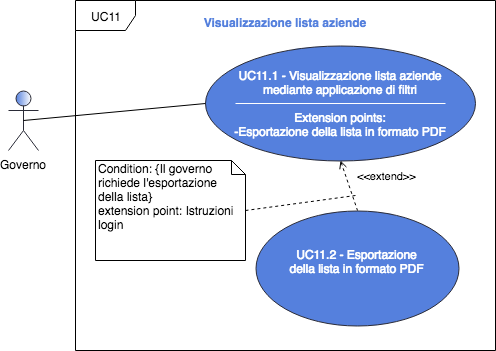
\includegraphics[width=10.5cm]{res/images/UC11Visualizzazione.png} %da adattare in larghezza
 	\centering
 	\caption{UC11 - Visualizzazione lista aziende}
 	
 \end{figure}
 \begin{itemize}
 	\item \textbf{Attori Primari}: governo;
 	\item \textbf{Descrizione}: il governo può vedere una lista dettagliata relativa alle aziende che hanno pagato o che devono ancora pagare per uno specifico trimestre;
 	\item \textbf{Scenario}: il governo richiede la lista delle aziende;
 	\item \textbf{Precondizione}: il governo non è in possesso di alcuna lista;
 	\item \textbf{Postcondizione}: il governo è in possesso di ciò che ha richiesto.
 \end{itemize}
 \subsubsection{UC11.1 - Visualizzazione lista aziende mediante l'applicazione di filtri}
 \begin{itemize}
 	\item \textbf{Attori Primari}: governo;
 	\item \textbf{Descrizione}: il governo può vedere una lista dettagliata in base ai filtri applicati ;
 	\item \textbf{Scenario}: il governo richiede la lista ad hoc delle aziende;
 	\item \textbf{Estensioni}:
 	\begin{itemize}
 		\item \textbf{UC11.2}: in seguito alla richiesta di esportazione della lista precedentemente creata ad hoc, il governo può ottonere tale file;
 	\end{itemize}
 	\item \textbf{Precondizione}: il governo non dispone della lista personalizzata delle aziende ed applica alcuni filtri nell'apposita sezione del sito;
 	\item \textbf{Postcondizione}: il governo è in possesso di una lista personalizzata secondo le proprie esigenze.
 \end{itemize}
 \subsubsection{UC11.2 - Esportazione della lista in formato PDF}
 \begin{itemize}
 	\item \textbf{Attori Primari}: governo;
 	\item \textbf{Descrizione}: il governo ottiene in formato PDF la lista precedentemente creata;
 	\item \textbf{Scenario}: il governo clicca sull'apposito pulsante per esportare la lista in PDF;
 	\item \textbf{Precondizione}: il governo ha ottenuto una lista secondo alcuni filtri e non è in possesso della versione PDF, pertanto clicca sull'apposito pulsante;
 	\item \textbf{Postcondizione}: il governo ora è in possesso della versione PDF della lista precedentemente filtrata.
 \end{itemize}
